\section{Study of Price as a Function of All Variables} % (fold)
\label{sec:study_of_price_as_a_function_of_all_variables}

In this section, we will first calculate a linear regression model 
that takes all variables of the dataset into account in order to
predict the price of the used car. In the following, we will use different 
methods do decide on which variables will be used for our ``final model''. 
Therefore, different factors will be taken into consideration, such as

\begin{itemize}
	\item the \emph{``R-squared''} value showing how well the predictions fit the actual data and detected \emph{high biais},
	\item factors making sure the data is not \emph{overfitting}, such as 
	\emph{BIC}, \emph{AIC} and \emph{adjusted ``R-squared''}
	\item and factors using cross-validation methods in order to check 
	whether the model is useful for data the model was not ``trained on'' 
	(\emph{BIC}, \emph{AIC})
\end{itemize}

\subsection{Prelimenary Selection of Different Models} % (fold)
\label{sub:prelimenary_selection_of_different_models}

The first model we want to test later is simply the model that uses all 
variables in order to predict the price: 

\begin{equation}\label{eq:model1}
	M_1 = lm(price \sim\ .)
\end{equation}

The second model is obtained by looking at the p-values of every input 
variable using:

\begin{lstlisting}[caption={summary() in R},label={lst:summary_func}]
	summary(Model1)
\end{lstlisting}

It can be seen that there are three variables that have a significant lower 
p-value than the other variables, being the \emph{age,km and ageop2}.
Therefore our second model is as follows:

\begin{equation}\label{eq:model2}
	M_2 = lm(price \sim\ age + km + ageop2)
\end{equation}

Our third model is achieved by using stepFunction: ``stepAIC''. 
This function calculates the \emph{AIC} value of the model at every step and 
removes all the variables, so that the remaining model has a lower AIC and  
therefore is a ``better fit''.
Using this method, we get the following model:

\begin{equation}\label{eq:model3}
	M_3 = lm(price \sim\ age + km + ageop2 + kop2)
\end{equation}

Our fourth and last model is achieved by using a model of preselected 
variables and executing the stepAIC function on this model whereas the 
``stepAIC'' function will build on a preselected choice of variables.
It is in some way a mixture of the methods used to obtain model2 and model3. 
We preselect the variables \emph{age, km} since they show by far the highest p-values (see listing \ref{lst:summary_func}). Applying the ``stepAIC'' function, we get: 

\begin{equation}\label{eq:model4}
	M_4 = lm(price \sim\ age + km + ageop2 + kop2)
\end{equation} 

This is the same model as model 3 and can therefore be discarded.

\subsection{Validation of the Models} % (fold)
\label{sub:validation_of_the_models}

First, we want to calculate the different \emph{``R-squared''} values to select models having low biases when predicting the data. 
For all three models we get similiar results

\begin{table}[ht]
\begin{center}
\begin{tabular}{ |c|c|c|c| } 
 \hline
 & $M_1$ & $M_2$ & $M_3$ \\ 
 \hline
 $R^2$ &  0.65833 & 0.64338 & 0.65581 \\ 
 \hline
\end{tabular}
\end{center}
\end{table}
% subsection validation_of_the_models (end)

The closer \emph{``R-squared''} is to 1, the better it is. Obviously, the 
first model has the one that is closest to one since it uses all the variables for its model. We can see though that all \emph{``R-squared''} are very close to each other and can therefore not yet determine the 
best model. We need more analysis. 

To get in-depth analysis, we will use the ``CV'' function of the package ``forecast''. This function calculates the \emph{BIC}, \emph{AIC}, \emph{AICc} and \emph{adjusted ``R-squared''} for every model and returns 
a so-called ``PRESS'' value that takes into consideration all the factors mention above in the first part of the section \ref{sec:study_of_price_as_a_function_of_all_variables} (especially the second and third factor). The comparable lowest ``PRESS'' value stands for 
the best model. The result of the ``CV'' function gave us:

\begin{figure}[H]
  \begin{center}
    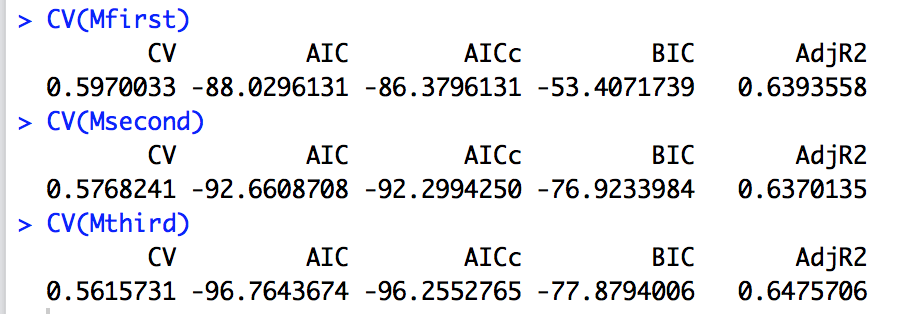
\includegraphics[scale=0.7]{./img/CV_analysis.png}
    \end{center}
  \caption{\textit{PRESS} anaysis of the models.}
  \label{fig:Scatter}
\end{figure}

As we can see, we get the lowest CV for the third model.

% subsection prelimenary_selection_of_different_models (end)

% section study_of_price_as_a_function_of_all_variables (end)

